\chapter{Aprendizado de Máquina}


AM pode ser altamente benéfico para solução de problemas complexos, é possível observar um ciclo de trabalho bem definido que está presente na solução de problemas por uma abordagem de Aprendizado de Máquina. As etapas gerais de projetos de AM são aquisição de dados, construção de modelo, análise, otimização e predição. Com estas cinco etapas é possível sair de um conjunto de dados e chegar as respostas desejadas através de cuidadosa seleção e processamento de dados. Passando pela construção e avaliação de um método eficaz até chegar a um modelo consistente com a necessidade do problema. Embora haja uma linearidade na execução desses processos é comum em projetos de AM revisitar estas etapas várias vezes. A imagem a seguir revela um ciclo de AM mais detalhado e que engloba as etapas previamente citadas ressaltando elementos importantes  \cite{real2013}: 

\begin{figure}[!h]
\centering
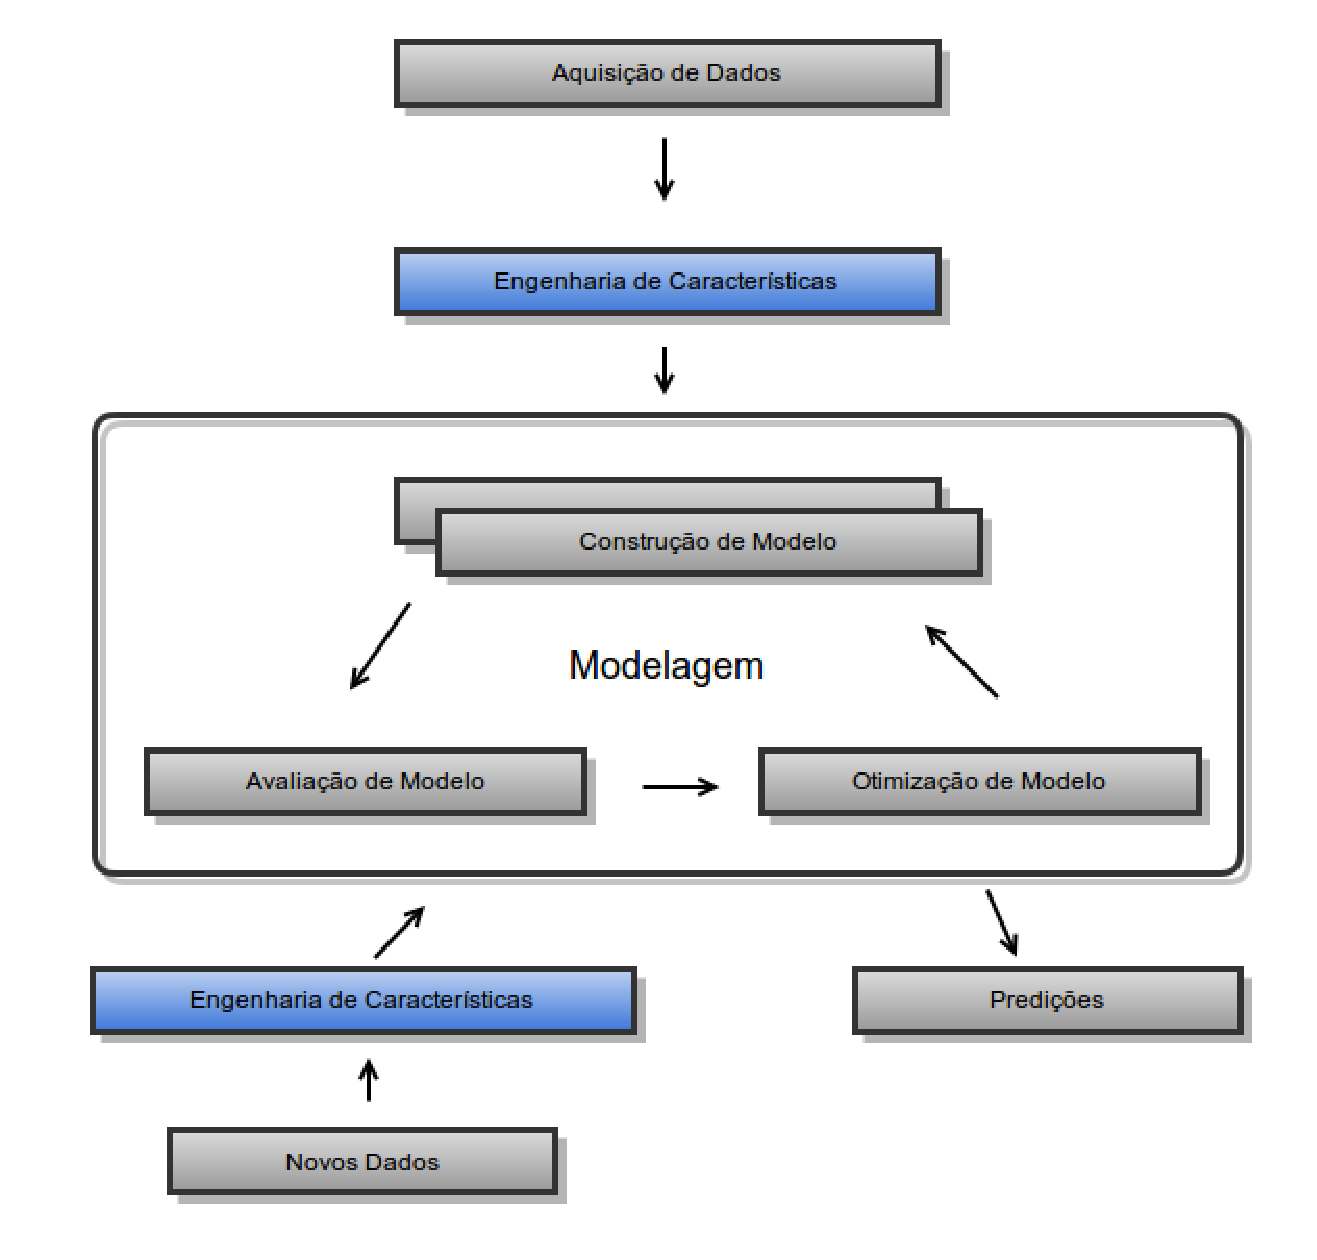
\includegraphics[keepaspectratio=true,scale=0.50]
{figuras/workflowml.eps}
\caption{Fluxo de Trabalho de AM}
\label{workflow_am}
\end{figure}

Este capítulo serve para detalhar os processos AM. A figura anterior mostra os ciclos de trabalho que acontecem até que o modelo esteja satisfatório com as expectativas de performance. Várias etapas podem ser repetidas até que o modelo esteja refinado o suficiente. A área central que corresponde a construção do modelo pode levar várias iterações e, as vezes, é necessário rever até mesmo a primeira etapa do ciclo, Aquisição dos Dados. As próximas seções deste capítulo seguem os processos descritos no fluxo de trabalho de AM.

\begin{enumerate}
\item Aquisição dos dados
\item Engenharia de Características
\item Construção do modelo
\item Avaliação e Otimização de Modelo
\item Predições
\end{enumerate}

\section{Aquisição dos dados}
Apesar de parecer trivial, definir a aquisição de dados como uma etapa do projeto de AM é extremamente importante e alguns cuidados especiais devem ser considerados para que as predições tenham um bom desempenho. O primeiro passo antes de começar o projeto de AM é saber qual a necessidade do mundo real que deve ser atendida. Este passo pode ser entendido como a necessidade de encontrar questões que envolvem uma variável de interesse (quem gostaria de comprar este produto, qual o significado deste áudio em linguagem natural, onde está a face humana nesta imagem,...) e o caminho pra solução que envolve variáveis independentes (histórico de compras dos usuários, mapeamento de sons para texto, características de faces humanas).

Nem sempre utilizar Aprendizagem de Máquina é a melhor resposta para solucionar os problemas do mundo real. É necessário avaliar com cuidado quais os objetivos da solução e qual o contexto do problema. Um grande indício de que o problema pode ser solucionado por AM é se ele possui algumas das seguintes características: Alta complexidade entre entradas e saídas, grande volume de dados, necessidade de generalização e necessidade de adaptabilidade a novos cenários. 

Os dados que servem como entrada para os processos de modelagem geralmente estão apresentados na forma de tabelas que possuem colunas e linhas. As colunas representam as características dos dados, como se fossem meta-dados, e as linhas representam instâncias dessas características. A tabela a seguir representa os tipos de dados que podem aparecer como característica de dados na Aprendizagem de Máquina \cite{guy2010}.

\begin{table}[h]
\centering
\caption{Tipos de Dados}
\vspace{0.5cm}
\begin{tabular}{r|lr}

\hline 
Tipo & Exemplo  \\ % Note a separação de col. e a quebra de linhas
\hline                               % para uma linha horizontal
Átomo Categórico        & Uma palavra na língua portuguesa \\
\hline   
Átomo Numérico & Valor de temperatura \\
\hline 
Átomo Ordinário           & Preferência cinematográfica (Número de Estrelas) \\
\hline 
Conjunto desordenado de números       & Sinais vitais(pulso, temperatura, pressão sanguínea)\\
\hline 
Conjunto desordenado de misturas     & Informação demográfica(raça, sexo, idade, renda)\\
\hline 
Sequência unidimensional de categóricos       & Documento de texto\\
\hline 
Sequência unidimensional de números       & Série Temporal Financeira\\
\hline 
Sequência bidimensional de números      & Imagem\\
\hline 
Sequência tridimensional de números       & Filme\\
\hline 
Grafo Arbitrário Categórico       & Árvore de Conversões\\
 \hline 
\end{tabular}
\end{table}

A figura a seguir é uma pequena seleção da base de dados que contém informações sobre os passageiros que estavam presentes no naufrágio do Titanic \cite{titanic2012}. 

\begin{figure}[!h]
\centering
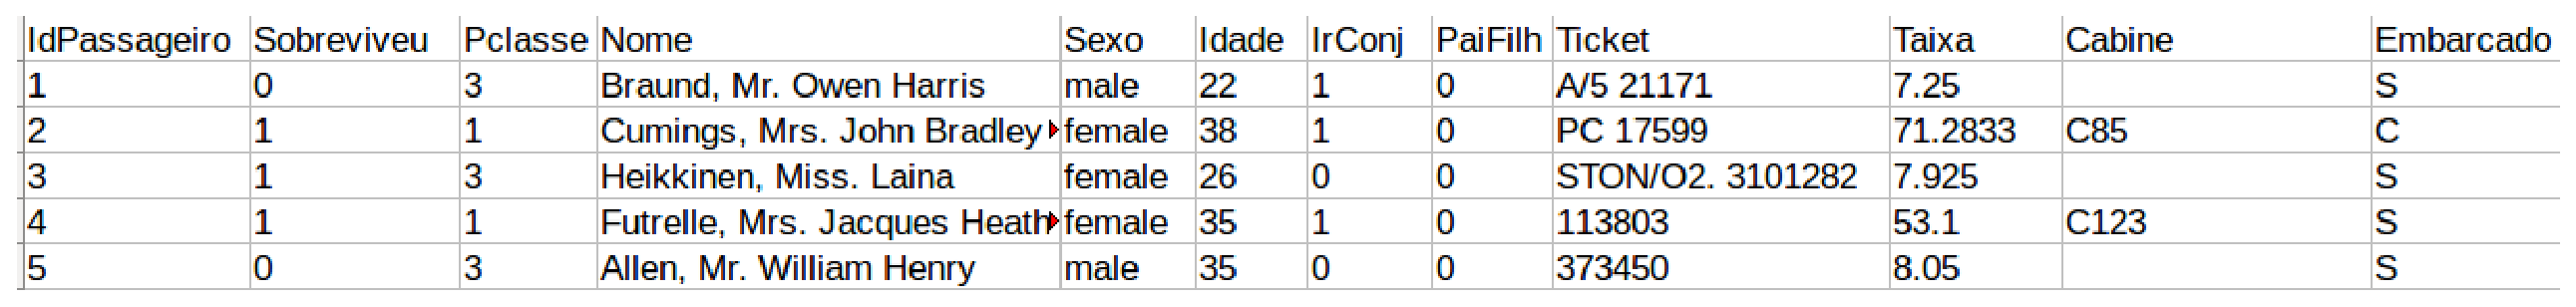
\includegraphics[keepaspectratio=true,scale=0.40]
{figuras/dataEg.eps}
\caption{Exemplo de Dados do Titanic}
\label{data_titatic}
\end{figure}

Cada linha corresponde as informações de um passageiro e cada coluna representa um tipo de informação deste passageiro. Esta base de dados foi criada com objetivo de tentar prever, através das informações de um passageiro, se ele sobreviveu ou não ao naufrágio. A base já contém a informação sobre a sobrevivência do passageiro. Muitos modelos são criados com base nas informações deste conjunto de dados, é possível fazer predições sobre a sobrevivência dos passageiros e comparar estes resultados com a informação real que já esta registrada nas tabelas. Por este motivo o conjunto de dados vem sendo usado de forma didática para AM, muitas pessoas o usam para validar seus modelos e há competições baseadas em predições com esta base \cite{titanic2011}. A enumeração a seguir explica qual o tipo de informação de cada coluna. 

\begin{enumerate}
\item IDPassageiro: Um átomo numérico que identifica unicamente cada passageiro.
\item Sobreviveu: Um átomo numérico que representa se a pessoa sobreviveu ou não ao naufrágio. Assume valor "1" para sobreviventes e "0" para não sobreviventes.
\item Pclasse: Átomo numérico que varia de "1" a "3", representa a classe do passageiro. "1" equivale a primeira classe, "2" a segunda classe e "3" a terceira.
\item Nome: Átomo categórico que representa o nome do passageiro.
\item Sexo: Átomo categórico que representa o sexo do passageiro.
\item Idade: Átomo numérico que representa a idade do passageiro.
\item IrConj: Átomo numérico que representa a soma da quantidade de irmãos e cônjuges do passageiro a bordo.
\item PaiFilh: Átomo numérico que representa a soma da quantidade de pais e filhos do passageiro a bordo.
\item Ticket: Átomo categórico que representa o número do ticket de embarque do passageiro.
\item Taixa: Átomo numérico que representa o preço da passagem paga pelo passageiro.
\item Cabine: Átomo categórico que representa o número da cabine do passageiro.
\item Embarcado: Átomo categórico que representa o porto de embarque do passageiro. "C"  para a cidade de Cherbourg, "Q"  para a cidade de Queesntown e "S"  para Southampton.
\end{enumerate}


É importante notar que nem todos os dados disponíveis são úteis para a resolução do problema. Qual seria a relevância do atributo \textbf{IDPassageiro} na resolução do problema? Este atributo é gerado automaticamente e está relacionado com a ordem dos registros no computador e não com uma característica real do passageiro. A decisão de escolher que dados são úteis para a solução do problema é um trabalho não trivial, que exige conhecimento do contexto do problema e repetidas iterações de otimização. Conhecendo o problema é possível descartar informações que não são relevantes, e tendo um modelo pronto é possível testar se determinada informação afeta ou não a performance da predição. Diminuir a quantidade de informações que entra no modelo pode ajudar no tempo em que as predições são feitas e também na performance do sistema em geral, isto se deve ao fato de que ter informações que não se relacionam com a variável de interesse aumenta o ruído do sistema, a figura 3 demonstra este fluxo de trabalho \cite{real2013}.

\begin{figure}[!h]
\centering
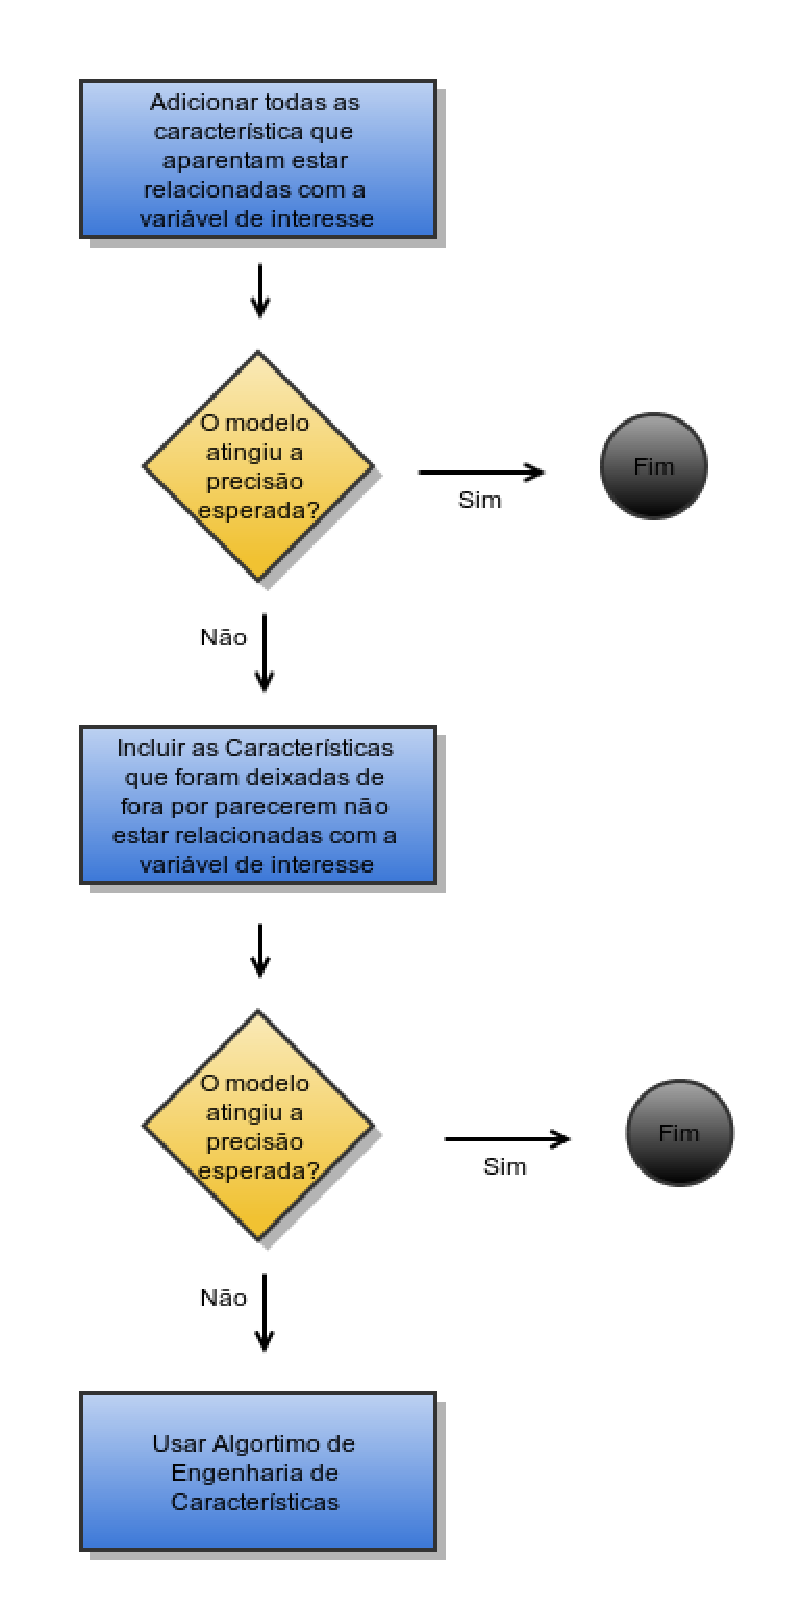
\includegraphics[keepaspectratio=true,scale=0.5]
{figuras/data_workflow.eps}
\caption{Fluxo de Trabalho da Seleção de Características}
\label{workflow_data}
\end{figure}

Se houver dúvida sobre a relação causal entre determinada variável e a saída do sistema é possível realizar duas execuções do modelo: Uma com a variável independente e outra sem. Se não houver melhora na predição esse é um sinal de que a informação pode ser descartada, caso haja queda na precisão, é um indício de que a variável independente tem relação causal com a variável de interesse.

Outro fator relevante na Aquisição de Dados é que a maioria dos modelos só aceitam entradas numéricas ou categóricas. Portanto é necessário transformar outros tipos de dados em entradas ideais por um processo chamado de Engenharia de Características, este processo será descrito a frente \cite{real2013}. 

Como é possível observar na pequena seleção da base de dados do Titanic, coluna 11 (Cabine) da Figura 2, existem algumas linhas que não possuem seu valor preenchido. Esse fenômeno é chamado de Dados Faltantes, do inglês Missing Data. É comum em diversas bases de dados encontrar informações faltantes, isso se deve a diversos motivos, como erro na hora da coleta ou perdas que acontecem com o tempo. Estas informações podem ser decisivas para que o modelo aprenda algum relacionamento novo e de acordo com os autores de \citeonline{anal2003} (em livre tradução) "Um problema relevante na qualidade dos dados é a presença de dados faltantes" e " ... o tratamento de dados faltantes deve ser feito com muito cuidado, de outra forma erro pode ser introduzido no conhecimento aprendido". 

Dados faltantes podem ser encontrados por diversos motivos dentro de uma base de dados, nem todos os motivos estão relacionados a erros humanos e é importante conhecer a origem de cada tipo de dado faltante para utilizar o método de tratamento correto. A enumeração a seguir demonstra os tipos de Dados Faltantes que podem existir de acordo com \cite{stat1987}.

\begin{enumerate}
\item Missing completely at random (MCAR):Perda completamente ao acaso. É o maior nível de randomicidade. Acontece quando a probabilidade de perda em um caso pode não depender nem dos valores que esse atributo assume nem do dado perdido em si. É naturalmente randômico e qualquer método de tratamento pode ser utilizado sem o risco de introduzir erro no aprendizado.
\item Missing at random (MAR): Perda ao acaso. Quando a probabilidade de perda pode depender dos valores que atributo pode assumir, mas não pode depender do dado perdido em si.
\item Not missing at random (NMAR): Perda ao não acaso. Neste caso pode existir algum motivo real para que a instância esteja perdida. A probabilidade de perda pode depender do valor que a instância do dado assume no momento.
\end{enumerate}

Muitos métodos são propostos para lidar com este problema, ainda de acordo com  R. J. Little e D. B. Rubin apud \citeonline{anal2003}, os métodos de tratamento para dados faltantes se enquadram em uma das três categorias a seguir:

\begin{enumerate}
\item Ignorar e descartar o dado: Consiste em descartar o dados faltantes. A primeira forma de fazer isso é descartar toda a tupla que contém algum dado faltante. Outra forma é avaliar a quantidade de dados faltantes em cada tupla e em cada coluna, depois disso eliminar as instâncias(tupla ou coluna) de acordo com extensão dos dados faltantes. Antes de deletar qualquer tupla ou atributo é necessário analisar a importância desse dado na performance geral do modelo. Atributos que são relevantes devem ser mantidos mesmo se seu nível de perda for muito alto. Este método só deve ser usado quando os dados faltantes são do tipo MCAR.
\item Estimação de Parâmetro: Neste caso todas as instâncias parecidas são analisadas e o dado faltante tem seu valor atribuído com um valor que possui alta similaridade com seus vizinhos.
\item Imputação: Consiste em uma série de métodos que visam atribuir valores faltantes com estimações. Busca-se encontrar relacionamentos entre o sistema e os dados faltantes, pode-se dizer que um novo processo de AM é empregado para estimar estes valores.
\end{enumerate}


\section{Engenharia de Características}

Características englobam informações de dados brutos que habilitam algoritmos de aprendizado de máquina a classificar um objeto desconhecido ou fazer uma estimativa nova \cite{brain2013}. Características não são simplesmente conjuntos de dados, elas carregam mais informações sobre o contexto do problema. São abstrações que estruturam conjuntos de informação para que estes fiquem mais próximos a conhecimentos do mundo real.   

Engenharia de Características, EC, é o processo de transformar dados nunca trabalhados em características que melhor representam o problema atacado para o modelo preditivo, resultando em uma precisão de modelo melhorada nos dados escondidos \cite{fe2014}. Em uma outra definição, "... engenharia de características é projetar manualmente como os dados de entrada x devem ser" \cite{tomas2014}. Existem tipos de dados que precisam ser trabalhos antes de serem utilizados por modelos. Dados do tipo sequencial e do tipo categórico geralmente precisam ser tratados, pois há modelos que não estão preparados para recebe-los em sua forma inicial. Portanto, dois principais processos são feitos na base de informações inicial: análise dos dados, buscando encontrar características que não estão explícitas e transformações de dados explícitos em formatos que sejam compatíveis com o modelo escolhido. EC visa responder a pergunta: Qual a melhor forma de representar o problema pelos meus dados?

No fluxograma do começo deste capítulo, Engenharia de Características aparece como uma etapa anterior a fase de modelagem e como um processo que serve para melhorar a acurácia da modelagem. EC está no centro do Aprendizado de Máquina, pois através dela é possível entender os dados por suas características. Ela ajuda a dominar o contexto do problema, o que agrega conhecimento no modelo de AM, aumentando assim a performance das modelagens. Por esse motivo, EC aparece em vários momentos do fluxo de Aprendizado de Máquina. Inicialmente é necessário tratar os dados para começar a modelagem, e posteriormente Engenharia de Características é usada para melhorar o desempenho do modelo até que se chegue a uma precisão aceitável. 

O fluxo da Engenharia de Características é iterativo por si só. Ele consiste em construir novas características e testar o desempenho do modelo com elas. A seguinte figura descreve este fluxo \cite{fe2014}:


\begin{figure}[!h]
\centering
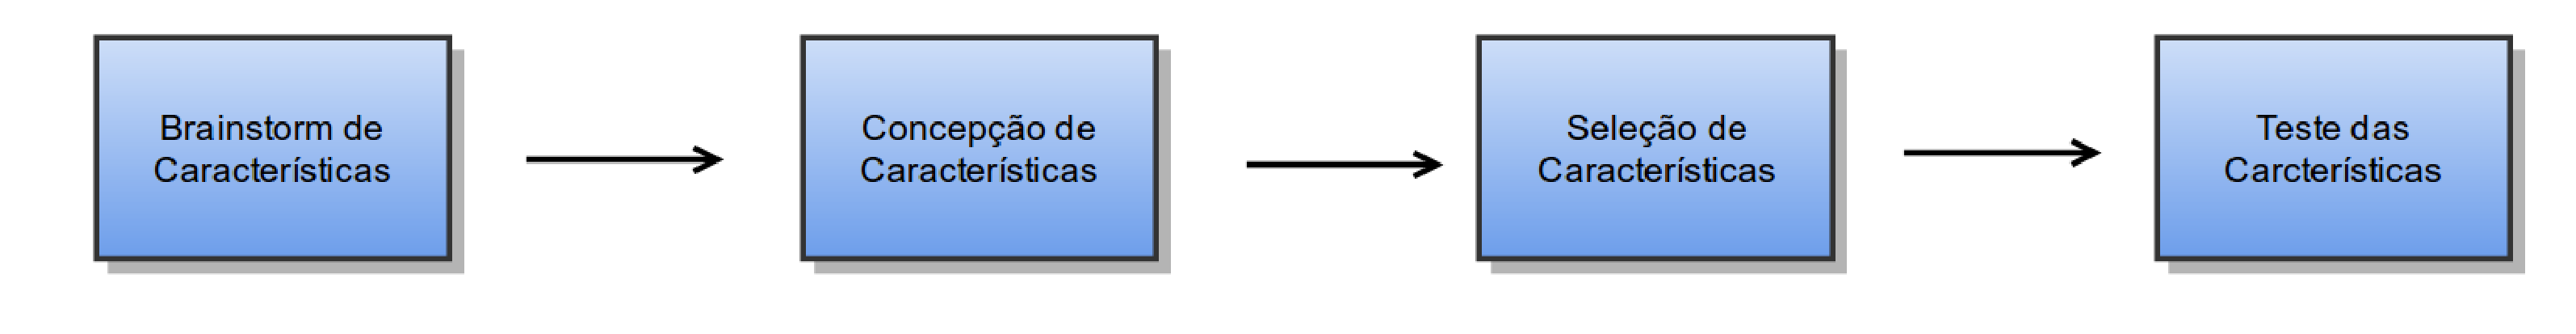
\includegraphics[keepaspectratio=true,scale=0.32]
{figuras/ecworflow.eps}
\caption{Fluxo de Trabalho de Engenharia de Características}
\label{workflow_ec}
\end{figure}

\begin{enumerate}
\item Brainstorm de Características: Nesta etapa um conjunto de possíveis características deve ser gerado.É necessário um aprofundamento no problema, através de meticulosa inspeção dos dados disponíveis e de experiências em casos similares. 
\item Concepção de Características: Consiste em construir características. É possível utilizar métodos automatizados de extração de características ou é possível criá-las manualmente através do conhecimento obtido na etapa anterior.
\item Seleção de Características: Nesta fase é feita uma escolha de um conjunto de características para serem testadas. É possível utilizar métodos de comparação entre as características existentes ou é possível escolher o conjunto  manualmente, de acordo com o que se conhece do problema.
\item Teste das Características: A última etapa é simples: basta introduzir as características no modelo e medir o desempenho.
\end{enumerate}

Usar Engenharia de Características sistematicamente pode aumentar a capacidade preditiva dos modelos, pois características novas são conhecimentos que poderiam não ser aprendidos naturalmente pelos algoritmos de AM. EC possibilita: Criar características que são mais relacionadas com a variável de interesse, permite a adição de informações externas relevantes dentro do modelo, habilita o uso de informações não estruturadas dentro dos modelos de AM e seleciona as características mais relevantes para a solução do problema \cite{real2013}. As próximas subseções mostram exemplos comuns de EC aplicadas no processo de AM.

\subsection{Decomposição de Atributos Categóricos}
Atributos categóricos assumem apenas um valor dentro de um conjunto de possibilidades de cada vez. Em uma tabela convencional apenas uma coluna é capaz de descrever este comportamento. Temos do exemplo do Titanic a coluna Sexo: 

\begin{figure}[!h]
\centering
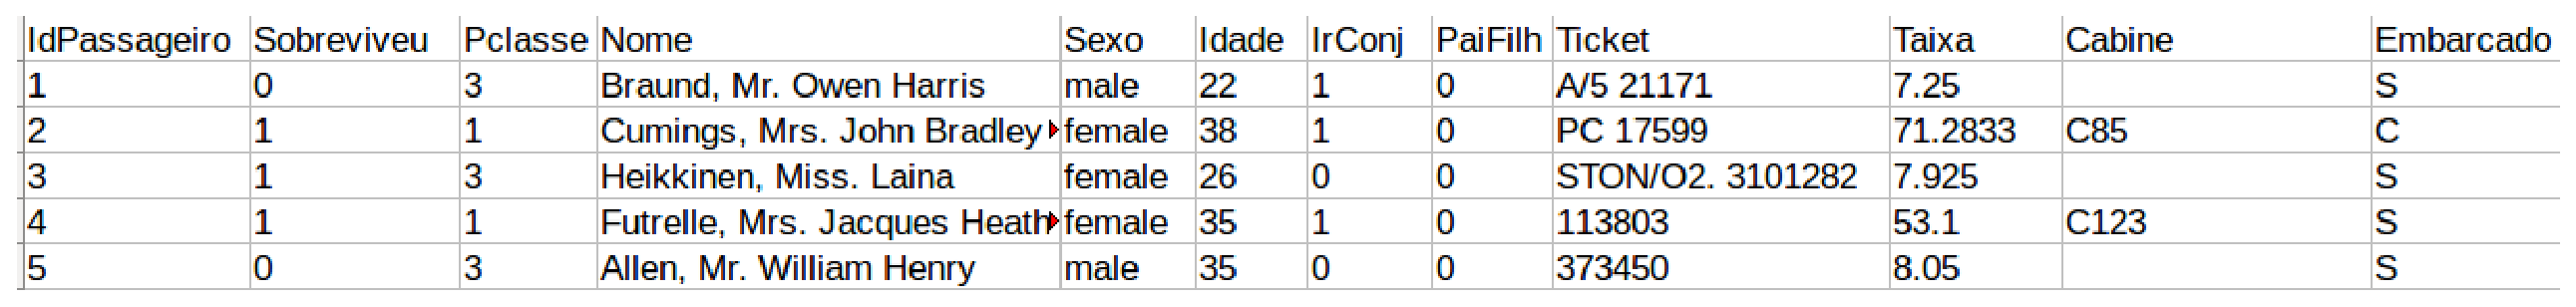
\includegraphics[keepaspectratio=true,scale=0.40]
{figuras/dataEg.eps}
\caption{Exemplo de Dados do Titanic}
\label{data_titatic}
\end{figure}

Cada pessoa pode ter como valor nesta coluna "male" para o sexo masculino e "female" para o sexo feminino. Muitos modelos não estão preparados para lidar com este tipo de dado. Em geral, modelos(algoritmos lineares, árvores de decisão...) precisam de informações numéricas atômicas para atuar de forma eficiente. A solução neste caso é criar mais categorias, uma coluna nova para cada valor de categoria que é possível assumir. No exemplo do Titanic é necessário abolir a coluna sexo e criar duas novas colunas: "émasculino" e "éfeminino". Estas colunas assumem um valor binário e são inversamente complementares. Isto quer dizer que se o registro diz respeito a um homem ele terá o valor "1" na coluna "émasculino" e o valor "0" na coluna "éfeminino". A mesma lógica segue para qualquer tipo de categoria, o valor positivo para a categoria desejada e o valor negativo para todas as outras possibilidades.

\subsection{Decomposição de Características}
Muitos bancos de dados possuem informação de hora em um formato de sequência de caracteres. Um exemplo de padrão desta forma é o ISO 8601, na forma: 2014-09-20T20:45:40Z. Existe muito conhecimento condensado em apenas uma sequência de letras. Através de EC é possível quebrar esta sequência em muitas outras colunas, tornando o conhecimento mais claro e aumentando a capacidade de aprendizagem do modelo. Este padrão pode ser quebrado em várias outras características, como: Ano, mês, dia, hora, minuto, segundo e turno do dia. Este método é comumente aplicado para vídeos e imagens, que são sequências de informação. Este método consiste na decomposição de uma característica complexa em várias outras mais simples.


\subsection{Características Derivadas}
Outro tipo de conhecimento que pode ser extraído vem da precisão de átomos numéricos. Em determinado banco de dados pode haver a informação da massa de um produto. Esta massa pode ser medida em várias casas decimais de gramas ou pode estar arredondada em valores inteiros de quilogramas. Ter estas informações separadas pode servir como catalisador da precisão do modelo, o processo de teste das características dirá se esta é uma boa característica ou não. Também é possível criar um atributo do tipo booliano para um limite de peso, isto é, se o produto possui mais do que cinco quilos recebe valor positivo nesta característica, se a massa for menor, recebe valor negativo.

É necessário ainda o cuidado com a seleção das características. Nem sempre uma grande quantidade de características é a melhor opção para o modelo, é  preciso selecionar os atributos mais relevantes para aumentar a acurácia da previsão. Mais características inseridas no modelo dão a capacidade de aprender novos relacionamentos. A maioria dos modelos possui uma etapa de treino, onde o conhecimento é aprendido e absorvido pelo algoritmo, e uma etapa de teste, onde o algoritmo usa o conhecimento aprendido para realizar predições no conjunto de testes. Se muitas características do conjunto de treino forem colocadas no modelo ele poderá ser incapaz de generalizar conhecimentos e atuar de forma eficaz no conjunto de testes. O nome deste fenômeno é sobre-ajustamento, do Inglês overfitting. Sobre-ajustamento gera resultados superestimados em modelos: predições que aparecem em um modelo, que é sobre-ajustado com base no conjunto de treinamento, não existem na realidade e por isso não se replicaram no conjunto de testes \cite{what2013}. A figura a seguir mostra um exemplo de sobre-ajuste \cite{real2013}.

\begin{figure}[!h]
\centering
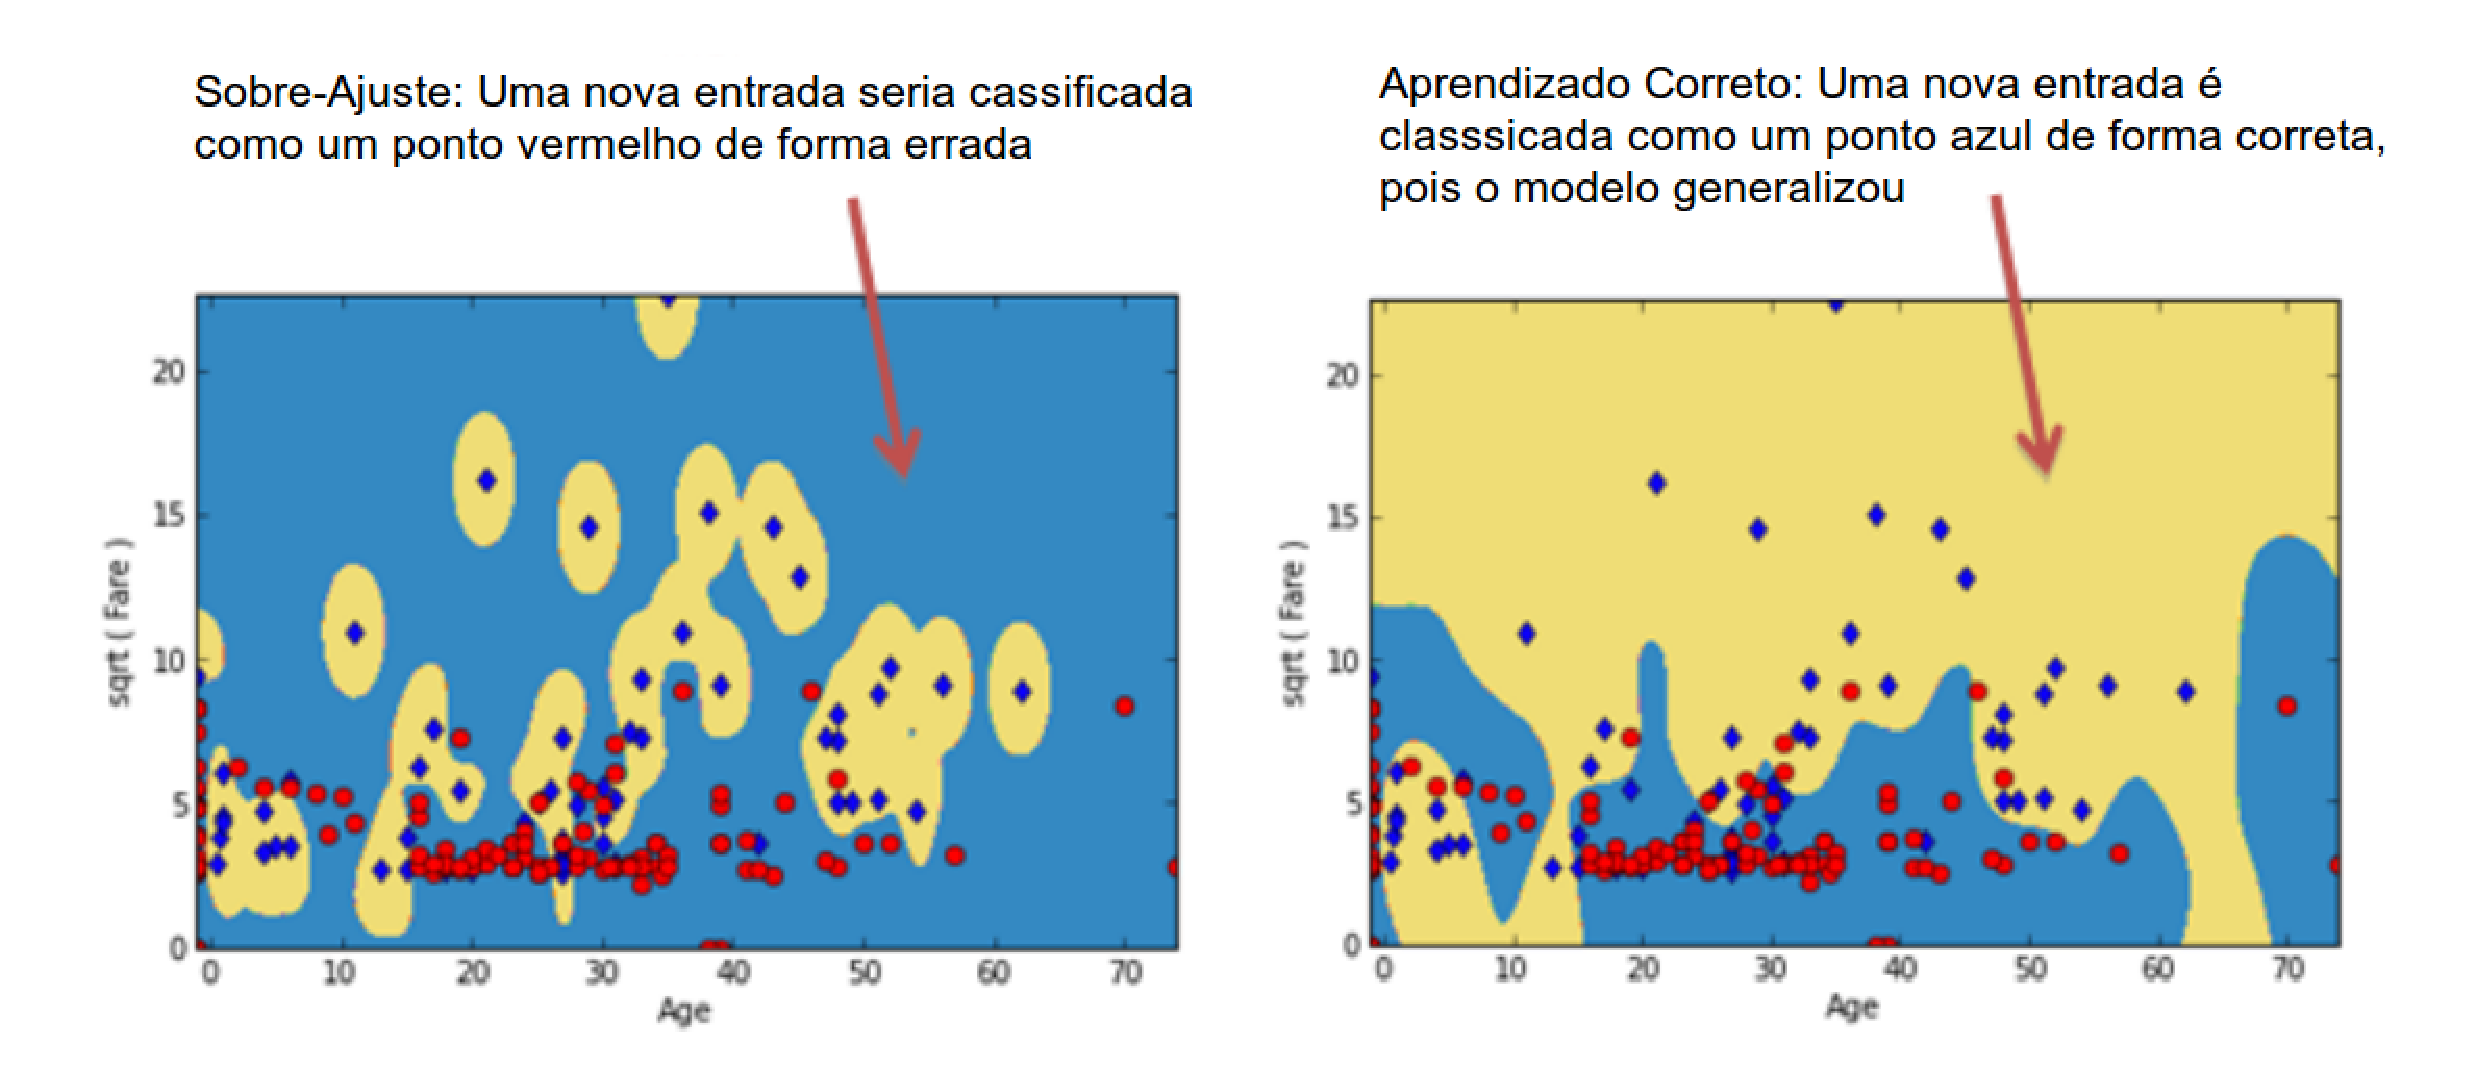
\includegraphics[keepaspectratio=true,scale=0.40]
{figuras/overfitting.eps}
\caption{Exemplo de Sobre-Ajustamento}
\label{over}
\end{figure}

No gráfico da esquerda o modelo sobre-ajustou, aprendeu características que são exclusivas do conjunto de treinamento. Provavelmente o modelo abstraiu ruídos do aprendizado. Do lado direito há um exemplo de aprendizado correto, o treinamento serviu para aprender características do mundo real e na aplicação houve generalização correta. É por este motivo que a seleção das características ideais é tão importante,a seguir são apresentados  métodos de seleção de características.

\begin{enumerate}
\item Força Bruta: O jeito mais simples de selecionar características é simplesmente seguir o fluxo de trabalho que foi apresentado no começo deste capítulo de forma manual. Escolher um conjunto de características e testar a validade destas no modelo. Uma das vantagens dos algoritmos de AM é a capacidade de lidar com um grande número de características. O problema deste método é que fazer a seleção de um grande número de características manualmente torna-se rapidamente inviável. 
\item Algoritmos de Seleção: Existem alguns algoritmos que são capazes de relacionar características com variável de interesse. Estes modelos possuem a seleção de características incorporada em sua concepção e são capazes de escolher as características mais relevantes. Embora estes métodos não sejam aplicáveis a todos os casos, pode ser interessante usá-los como um norteador para realizar a seleção por outras vias. 
\item Adição Iterativa: Este método consiste em partir de um conjunto vazio de características e adicionar todas as características que foram levantadas de forma sistemática, de uma a uma, e testar a precisão do modelo. A parada só acontece quando todas as características foram adicionadas, ou a precisão desejada foi alcançada ou o conjunto de características chegou a um tamanho máximo pré-determinado.
\item Remoção Iterativa: Este método parte de um conjunto que contém todas as características levantas, remove uma de cada vez e a cada iteração e testa a performance do modelo. A parada só acontece quando todas as características foram removidas, ou a precisão desejada foi alcançada ou o conjunto de características chegou a um tamanho mínimo pré-determinado.
\end{enumerate}

Seleção de características pode ser usada não apenas para evitar sobre-ajustamento e deixar o modelo mais leve. É possível construir um modelo de AM apenas para chegar a etapa de seleção das características, pois nesta etapa é possível obter conhecimento valioso sobre o mundo real: Quais as características tem maior relacionamento com a variável de interesse. Apenas esse conhecimento já é suficiente para aplicar grandes mudanças no mundo real. Usando uma base que relaciona características com pacientes de câncer é possível descobrir quais as características que são mais decisivas para o desenvolvimento de um tipo de câncer \cite{real2013}.

\section{Construção do modelo}
Depois de compreender o contexto do problema e passar um tempo definindo características na base de dados é hora de construir um modelo de predição apropriado. AM busca encontrar relacionamentos e padrões que estão dentro do conjunto de dados. Através de métodos matemáticos e computacionais é possível realizar esta tarefa. O processo de descoberta dos conhecimentos ocultos nos dados é atingido através do uso do modelo. Nesta etapa de construção do modelo, é necessário aplicar o que foi descoberto sobre as características dos dados e sobre o os objetivos da solução para escolher o modelo adequado. Existem vários métodos que podem ser utilizados para revelar os relacionamentos ocultos nos dados. Os métodos podem ser simples ou complexos, indo desde de regressões lineares até redes neurais que possuem centenas de neurônios. O objetivo desta seção é descrever características de diversos tipos de modelos, a relação entre necessidades do problema e características dos modelos é que indica os possíveis métodos adequados para atingir a solução. 

A seguinte equação serve muito bem para ilustrar o objetivo de um modelo de AM: \textbf{ Y = f(X) + e}. \textbf{Y} corresponde as predições, que é o resultado final do uso do modelo. \textbf{X} corresponde a todas as entradas que são usadas no modelo, estas informações vem da base de dados e já passaram pela etapa de pré-processamento e Engenharia de Características nas fases anteriores. O conjunto \textbf{X} são os registros reais, os métodos de AM são capazes de utilizar estas informações e extrair conhecimentos relevantes para a estimação de \textbf{Y}. Estes  métodos são representados por \textbf{f(X)}, onde \textbf{f()} é a técnica de modelagem que gera as predições baseadas nas entradas do sistema. O último elemento da equação é o erro \textbf{e}. Este erro determina a precisão da predição, de forma que, se o erro chegar a 0 a precisão é total. Este erro é advindo de várias fontes, algumas delas são: Medições imperfeitas, dados faltantes e super ajustamento \cite{real2013}.

Depois de ter uma boa estimativa para a função \textbf{f(X)} é possível realizar duas tarefas distintas: predição e inferência. Predições são o resultado direto da aplicação do modelo. Quando coloca-se um novo valor de \textbf{X}, que nunca foi visto antes, como entrada do modelo, a resposta da equação é equivalente a uma predição da realidade. Inferência é algo mais profundo, é entender os motivos dos relacionamentos entre as entradas e as saídas do modelo. Como citado anteriormente, Engenharia de Características pode ser usada para realizar inferências, pois uma inferência diz o quanto uma variável relaciona-se com o resultado final \cite{real2013}. 

Existem dois tipos de modelos de Aprendizado de Máquina, paramétrico e não-paramétrico. A diferença entre eles é que os modelos paramétricos assumem que a solução possui uma forma pré-definida, isto é, estes modelos tentam descobrir o formato da função \textbf{f(X)} assumindo que ela possui um formato de curva previamente conhecido. Um modelo caracteristicamente paramétrico é a regressão linear, este método assume que a função \textbf{f(X)} é uma combinação linear do vetor de entrada, \textbf{X}, com parâmetros numéricos. Métodos não-paramétricos não fazem nenhuma pré suposição com relação ao formato geométrico da função de estimativa, estes métodos mapeiam os parâmetros de entrada às saídas. Métodos paramétricos geralmente são mais fáceis de interpretar, mas possuem performance inferior a métodos não paramétricos. Métodos não-paramétricos são difíceis de interpretar, mas são uma forma de solução mais direta e não fazem pré-suposições, que podem estar erradas \cite{on2014}.

Problemas de Aprendizado de Máquina podem cair em duas categorias: Supervisionado e Não-Supervisionado. No caso supervisionado, o modelo de AM recebe um conjunto de dados de treinamento rotulado e faz predições para pontos que não possuem rótulo. Neste caso o algoritmo utiliza o rótulo de cada entrada para refinar o aprendizado, fazendo com que as características de cada entrada sejam relacionadas com o rótulo que ela possui. No caso de aprendizado não-supervisionado, o modelo recebe apenas dados que não possuem rótulo. Neste caso, o modelo é capaz de agrupar os dados de entrada em categorias, mas ele não possui conhecimento para afirmar o que estes grupos são no mundo real \cite{foundations2012}. A vantagem da utilização de aprendizagem supervisionada é que há conhecimento extra inserido por especialistas, isto dá mais sentido aos modelos deixando claro o que cada previsão representa no mundo real. As vezes os rótulos que acompanham os dados podem estar errados, e isto aumenta o ruído do sistema. Uma das vantagens da abordagem não supervisionada é não depender de rótulos, diminuindo o erro que vem de entradas classificadas de maneira errônea. 

Existem duas principais abordagens para aprendizado não-supervisionado: agrupamento e redução de dimensionalidade. O agrupamento consiste em descobrir qual é a maneira natural que os dados de entrada se agrupam, basicamente o que o modelo faz é unir as entradas em grupos distintos de acordo com a semelhança que eles possuem entre si. A redução de dimensionalidade consiste em diminuir a complexidade das entradas. Isto é atingido quando características mais relevantes são selecionadas de acordo com a variabilidade dos dados.





\section{Avaliação e Otimização de Modelo}
\section{Predições}


